%2multibyte Version: 5.50.0.2960 CodePage: 1252
%\usepackage{mathpazo}


\documentclass[smaller]{beamer}\usepackage[]{graphicx}\usepackage[]{color}
% maxwidth is the original width if it is less than linewidth
% otherwise use linewidth (to make sure the graphics do not exceed the margin)
\makeatletter
\def\maxwidth{ %
  \ifdim\Gin@nat@width>\linewidth
    \linewidth
  \else
    \Gin@nat@width
  \fi
}
\makeatother

\definecolor{fgcolor}{rgb}{0.345, 0.345, 0.345}
\newcommand{\hlnum}[1]{\textcolor[rgb]{0.686,0.059,0.569}{#1}}%
\newcommand{\hlstr}[1]{\textcolor[rgb]{0.192,0.494,0.8}{#1}}%
\newcommand{\hlcom}[1]{\textcolor[rgb]{0.678,0.584,0.686}{\textit{#1}}}%
\newcommand{\hlopt}[1]{\textcolor[rgb]{0,0,0}{#1}}%
\newcommand{\hlstd}[1]{\textcolor[rgb]{0.345,0.345,0.345}{#1}}%
\newcommand{\hlkwa}[1]{\textcolor[rgb]{0.161,0.373,0.58}{\textbf{#1}}}%
\newcommand{\hlkwb}[1]{\textcolor[rgb]{0.69,0.353,0.396}{#1}}%
\newcommand{\hlkwc}[1]{\textcolor[rgb]{0.333,0.667,0.333}{#1}}%
\newcommand{\hlkwd}[1]{\textcolor[rgb]{0.737,0.353,0.396}{\textbf{#1}}}%
\let\hlipl\hlkwb

\usepackage{framed}
\makeatletter
\newenvironment{kframe}{%
 \def\at@end@of@kframe{}%
 \ifinner\ifhmode%
  \def\at@end@of@kframe{\end{minipage}}%
  \begin{minipage}{\columnwidth}%
 \fi\fi%
 \def\FrameCommand##1{\hskip\@totalleftmargin \hskip-\fboxsep
 \colorbox{shadecolor}{##1}\hskip-\fboxsep
     % There is no \\@totalrightmargin, so:
     \hskip-\linewidth \hskip-\@totalleftmargin \hskip\columnwidth}%
 \MakeFramed {\advance\hsize-\width
   \@totalleftmargin\z@ \linewidth\hsize
   \@setminipage}}%
 {\par\unskip\endMakeFramed%
 \at@end@of@kframe}
\makeatother

\definecolor{shadecolor}{rgb}{.97, .97, .97}
\definecolor{messagecolor}{rgb}{0, 0, 0}
\definecolor{warningcolor}{rgb}{1, 0, 1}
\definecolor{errorcolor}{rgb}{1, 0, 0}
\newenvironment{knitrout}{}{} % an empty environment to be redefined in TeX

\usepackage{alltt}
%%%%%%%%%%%%%%%%%%%%%%%%%%%%%%%%%%%%%%%%%%%%%%%%%%%%%%%%%%%%%%%%%%%%%%%%%%%%%%%%%%%%%%%%%%%%%%%%%%%%%%%%%%%%%%%%%%%%%%%%%%%%%%%%%%%%%%%%%%%%%%%%%%%%%%%%%%%%%%%%%%%%%%%%%%%%%%%%%%%%%%%%%%%%%%%%%%%%%%%%%%%%%%%%%%%%%%%%%%%%%%%%%%%%%%%%%%%%%%%%%%%%%%%%%%%%
\usepackage{amssymb}
\usepackage{amsmath}
\usepackage{graphicx}
\usepackage{hyperref}
\usepackage{multimedia}
\usepackage{epstopdf}
\usepackage{color}
\usepackage{tikz}


\setcounter{MaxMatrixCols}{10}
\newtheorem{remark}{Remark}[section]
\newtheorem{proposition}{Proposition}[section]
\newtheorem{interpretation}{Interpretation}[section]
\newtheorem{goal}{Goal}[section]
\newtheorem{statement}{Statement}[section]
\newtheorem{aes}{Aim \& Scope}[section]
\newtheorem{exercise}{Exercise}[section]
\renewcommand{\Pr}{P}

\newcommand{\mbf}[1]{\mathbf{#1}}
\newcommand{\beq}{\begin{equation}}
\newcommand{\eeq}{\end{equation}}
\newcommand{\bea}{\begin{eqnarray}}
\newcommand{\eea}{\end{eqnarray}}
\newcommand{\ba}{\begin{array}}
\newcommand{\ea}{\end{array}}
\newcommand{\bi}{\begin{itemize}}
\newcommand{\ei}{\end{itemize}}
\newcommand{\ben}{\begin{enumerate}}
\newcommand{\een}{\end{enumerate}}
\newcommand{\nn}{\nonumber}
\newcommand{\N}{\mathcal{N}}

\newenvironment{stepenumerate}{\begin{enumerate}[<+->]}{\end{enumerate}}
\newenvironment{stepitemize}{\begin{itemize}[<+->]}{\end{itemize} }
\newenvironment{stepenumeratewithalert}{\begin{enumerate}[<+-| alert@+>]}{\end{enumerate}}
\newenvironment{stepitemizewithalert}{\begin{itemize}[<+-| alert@+>]}{\end{itemize} }
\usetheme{Madrid}


%%%%%%%%%%%%%%%%%%%%%%%%%%%%%%%%%%%%%%%%%%%%%%%%%%%%%%%%%%%%%%%%%%%%%%%%%%%%%%%
% GSEM COLORS
%%%%%%%%%%%%%%%%%%%%%%%%%%%%%%%%%%%%%%%%%%%%%%%%%%%%%%%%%%%%%%%%%%%%%%%%%%%%%%%
\definecolor{darkGSEM}{RGB}{70,95,127}
\definecolor{darkGSEM2}{RGB}{40,80,150}
\definecolor{GSEM}{RGB}{96,121,153} % GSEM 10% lighter

%%% Global colors
\setbeamercolor*{palette primary}{use=structure,fg=white,bg=darkGSEM}
\setbeamercolor*{palette quaternary}{use=structure,fg=white,bg=darkGSEM!90}
\setbeamercolor{frametitle}{fg=white,bg=GSEM!80}

%%% TOC colors
\setbeamercolor{section in toc}{fg=darkGSEM}

%%% itemize colors
\setbeamertemplate{itemize items}[circle]
\setbeamercolor{itemize item}{fg=darkGSEM2}
\setbeamercolor{itemize subitem}{fg=darkGSEM2}
\setbeamercolor{itemize subsubitem}{fg=darkGSEM2}


%%% enumerate colors
\setbeamercolor{item projected}{fg=white,bg=GSEM}
\setbeamertemplate{enumerate item}{\insertenumlabel.}
\setbeamercolor{enumerate item}{fg=darkGSEM2}
\setbeamercolor{enumerate subitem}{fg=darkGSEM2}
\setbeamercolor{enumerate subsubitem}{fg=darkGSEM2}


\AtBeginSection[]
{
  \begin{frame}
    \frametitle{Outline}
    \tableofcontents[currentsection]
  \end{frame}
}

\AtBeginSubsection[]
{
  \begin{frame}
    \frametitle{Outline}
    \tableofcontents[currentsubsection]
  \end{frame}
}



%%%%%%%%%%%%%%%%%%%%%%%%%%%%%%%%%%%%%%%%%%%%%%%%%%%%%%%%%%%%%%%%%%%%%%%%%%%%%%%%
% R Chunk Options and Packages
%%%%%%%%%%%%%%%%%%%%%%%%%%%%%%%%%%%%%%%%%%%%%%%%%%%%%%%%%%%%%%%%%%%%%%%%%%%%%%%%




%%%%%%%%%%%%%%%%%%%%%%%%%%%%%%%%%%%%%%%%%%%%%%%%%%%%%%%%%%%%%%%%%%%%%%%%%%%%%%%%
\IfFileExists{upquote.sty}{\usepackage{upquote}}{}
\begin{document}

\title[S110015]{Probability 1}
\subtitle{Chapter 05 : Continuous Random Variables - Part 2}
\author[Flores-Agreda, La Vecchia]{Dr. Daniel Flores-Agreda, \\[0.5em] \tiny{(based on the notes of Prof. Davide La Vecchia)}}
\date{Spring Semester 2021}

\begin{frame}
\titlepage
\end{frame}


\begin{frame}{Objectives}

\begin{itemize}
\item End exploration of the main properties of the Normal Distribution \bigskip
\item Explore other important Continuous Distributions
\end{itemize}

\end{frame}

\begin{frame}{Outline}
\tableofcontents
\end{frame}


%%%%%%%%%%%%%%%%%%%%%%%%%%%%%%%%%%%%%%%%%%%%%%%%%%%%%%%%%%%%%%%%%%%%%%%%%%%%%%%
\section{Gaussian Distribution (continued)}
%%%%%%%%%%%%%%%%%%%%%%%%%%%%%%%%%%%%%%%%%%%%%%%%%%%%%%%%%%%%%%%%%%%%%%%%%%%%%%%

\begin{frame}
  \begin{center}
  \Large Previously, on ``Probability 1'' \dots
  \end{center}
\end{frame}


\begin{frame}{\secname}
We explored the Normal PDF

$$
\phi_{(\mu,\sigma)}(x) =\frac{1}{\sqrt{2\pi \sigma ^{2}}}\exp{ \left\{ -\frac{1%
  }{2\sigma ^{2}}\left( x-\mu \right) ^{2}\right\}}~~-\infty<x<\infty\,
$$

\bigskip

And the Normal CDF
$$
\Phi_{(\mu,\sigma)}(x) =\int_{-\infty}^{x} \frac{1}{\sqrt{2\pi \sigma ^{2}}}\exp{ \left\{ -\frac{1%
  }{2\sigma ^{2}}\left(t-\mu \right) ^{2}\right\}}dt
$$

\end{frame}

\begin{frame}{\secname}
We saw that to evaluate the CDF, we could make use of the \textbf{Standard Normal CDF}
using \textbf{integration by substitution} $\color{blue}{s = \frac{t-\mu}{\sigma}}$

\begin{align*}
P(X \leq x) =
\Phi_{(\mu,\sigma)}(x)
&=
\int_{-\infty}^{x} \frac{1}{\sqrt{2\pi \sigma ^{2}}}\exp{\left\{-\frac{1}{2\sigma ^{2}}\left(t-\mu \right) ^{2}\right\}}dt\\
&=
\int_{-\infty}^{{\color{blue}{\frac{x-\mu}{\sigma}}}}\frac{1}{\sqrt{2\pi}}\exp{\left\{ -\frac{1
  }{2}{\color{blue}{s}}^{2}\right\}}d{\color{blue}{s}}\\
\Phi_{(\mu,\sigma)}(x)  &= \Phi\left(\frac{x-\mu}{\sigma}\right)
\end{align*}

\end{frame}


\begin{frame}{\secname}

  Last class we said that, the Normal PDF is \textbf{Symmetric}

  $$\phi_{(\mu,\sigma)}(-x) = \phi_{(\mu,\sigma)}(x)$$

\begin{knitrout}
\definecolor{shadecolor}{rgb}{0.969, 0.969, 0.969}\color{fgcolor}

{\centering 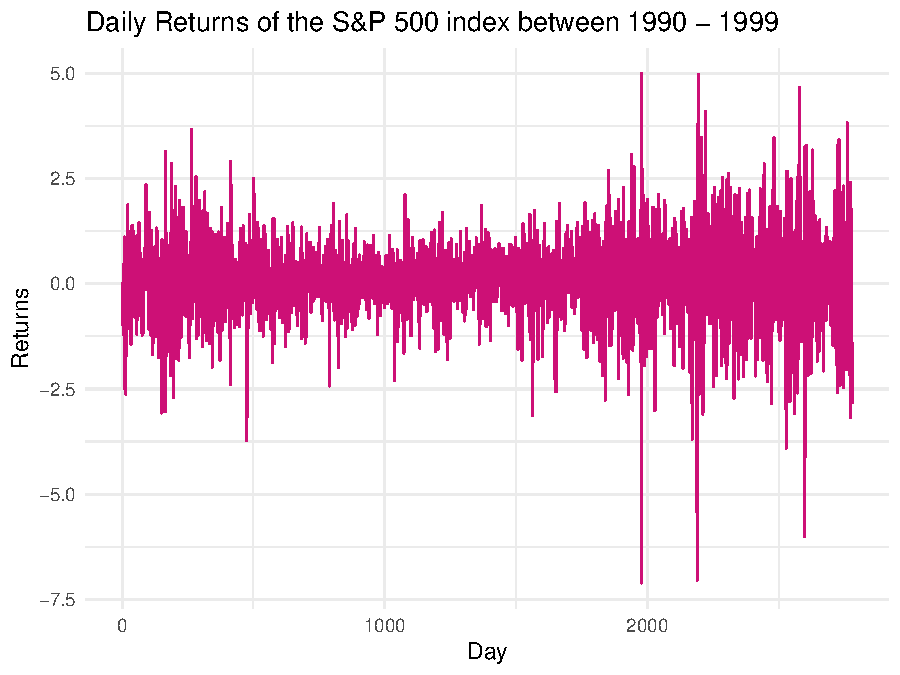
\includegraphics[width=0.5\linewidth]{figure/unnamed-chunk-2-1} 

}



\end{knitrout}

\end{frame}


\begin{frame}{\secname}

  Of course, the \textbf{Standard} Normal PDF is also \textbf{Symmetric}

  $$\phi(-x) = \phi(x)$$
\begin{knitrout}
\definecolor{shadecolor}{rgb}{0.969, 0.969, 0.969}\color{fgcolor}

{\centering 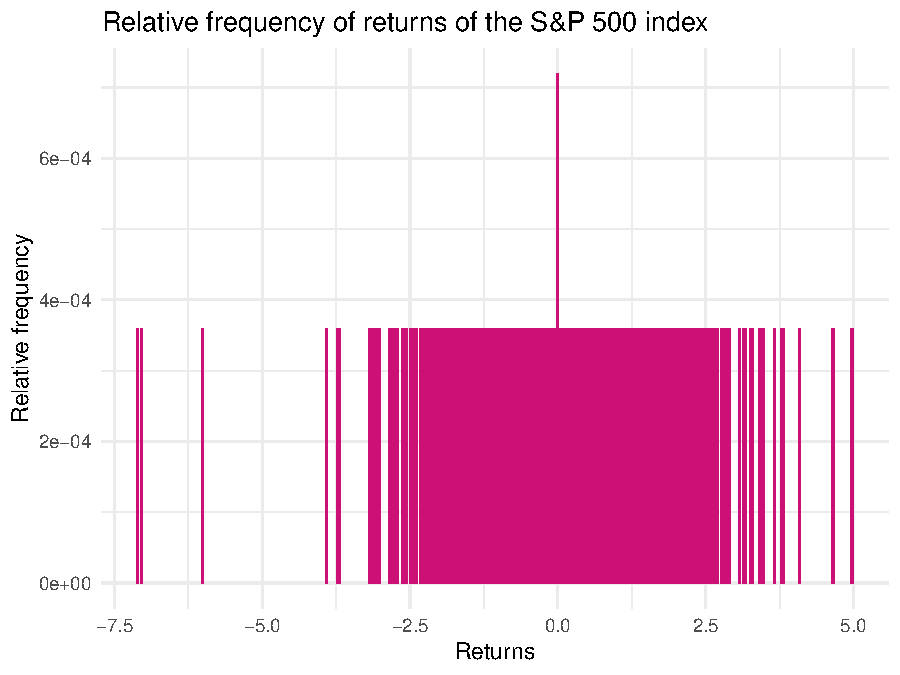
\includegraphics[width=0.5\linewidth]{figure/unnamed-chunk-3-1} 

}



\end{knitrout}
\end{frame}

\begin{frame}{\secname}

  \textbf{Symmetry} of the PDF implies that the CDF can be computed as

  $$\Phi(-x) = 1-\Phi(x)$$


\only<1-1>{
\begin{knitrout}
\definecolor{shadecolor}{rgb}{0.969, 0.969, 0.969}\color{fgcolor}

{\centering 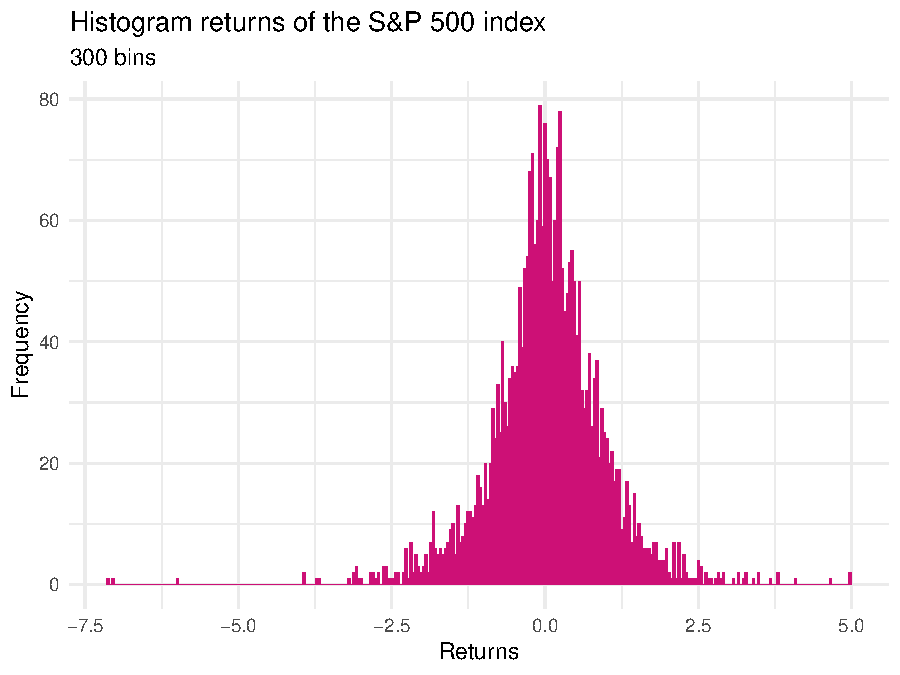
\includegraphics[width=0.5\linewidth]{figure/unnamed-chunk-5-1} 

}



\end{knitrout}
}
\only<2-2>{
\begin{knitrout}
\definecolor{shadecolor}{rgb}{0.969, 0.969, 0.969}\color{fgcolor}

{\centering 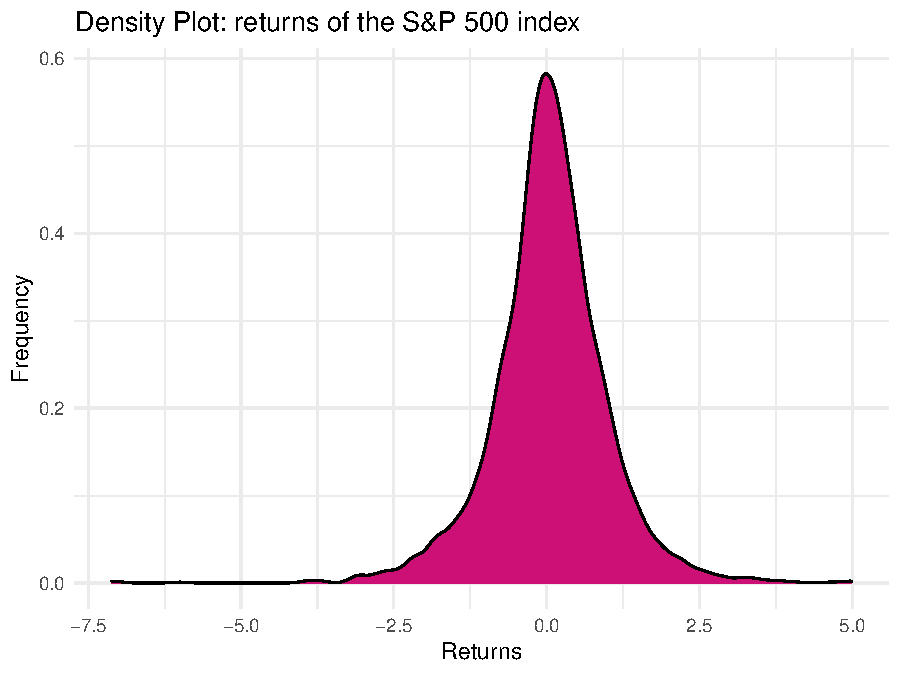
\includegraphics[width=0.5\linewidth]{figure/unnamed-chunk-6-1} 

}



\end{knitrout}
}
\only<3-3>{
\begin{knitrout}
\definecolor{shadecolor}{rgb}{0.969, 0.969, 0.969}\color{fgcolor}

{\centering 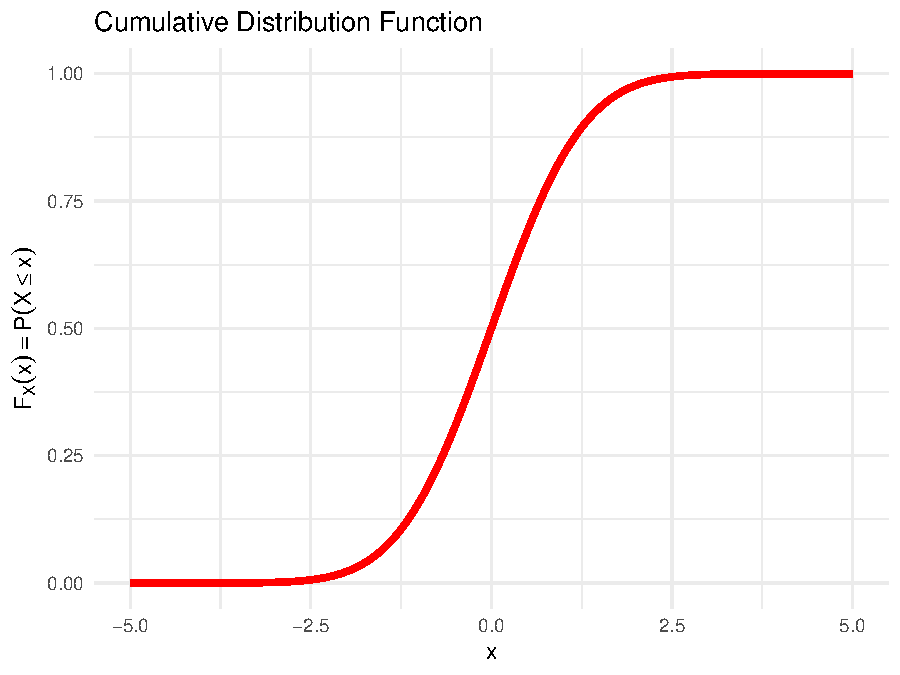
\includegraphics[width=0.5\linewidth]{figure/unnamed-chunk-7-1} 

}



\end{knitrout}
}
\end{frame}


\begin{frame}{\secname}
  % Thus statements about a Normal random variable can always be translated into equivalent statements about a standard Normal random variable, and vice versa.

We can \textbf{shift and scale} any Normal Random Variable $X$ and reach a \textbf{Standard Normal Random Variable} $Z$

$$X\sim \N\left( \mu ,\sigma ^{2}\right)\Longleftrightarrow Z=\frac{X-\mu}{\sigma}\sim \N\left( 0,1\right)$$

\pause

  \begin{itemize}
  \item We can always \textbf{transform from $X$ to $Z$}
  \begin{equation*}
  Z=\frac{X-\mu }{\sigma } \ (\text{for the random variable}) \quad\mbox{and}\quad z=\frac{x-\mu }{\sigma }\,  \ (\text{for its values}) ,
  \end{equation*}
  \item and \textbf{return back to $X$ by a `re-scaling' and `re-shifting'}:
  \begin{equation*}
  X=\sigma Z+\mu  \ (\text{for the random variable}) \quad\mbox{and}\quad x=\sigma z+\mu\, \ (\text{for its values}).
  \end{equation*}
  \end{itemize}
\pause

\begin{remark}[Implication]
Statements about a Normal Random Variable can always be translated into equivalent statements about a standard Normal Random Variable, (and vice-versa).
\end{remark}
\end{frame}

\begin{frame}{\secname}
  In particular, the \textbf{CDF of any Normal Random Variable} $X\sim \N(\mu, \sigma^2)$, can
  be \textbf{computed} with a \textbf{Standard CDF}

  \begin{align*}
  P(\{ X\leq x\}) &=
  P\left(\left\{\underbrace{\frac{X-\mu}{\sigma}}_Z\leq \underbrace{\frac{x-\mu}{\sigma}}_{z}\right\}\right) \\
  &= P(\{ Z\leq z\}) \\
  P(\{ X\leq x\})&= \Phi(z)
  \end{align*}
\end{frame}

\begin{frame}{\secname}
Moreover, we can also compute the probabilities of any interval for $X\sim \N\left( \mu ,\sigma ^{2}\right)$ with the \textbf{Standard CDF}

\begin{align*}
  \Pr(\{x_1<X\leq x_2\}) &=
  \Pr\left(\left\{\frac{x_1-\mu}{\sigma}<\frac{X-\mu}{\sigma}\leq \frac{x_2-\mu}{\sigma}\right\}\right) \\
  &= \Pr(\{z_1<Z\leq z_2\})\\
  &= \Pr(\{Z\leq z_2\}) - \Pr(\{Z\leq z_1\})\\
  \Pr(\{x_1<X\leq x_2\}) &= \Phi(z_2)-\Phi(z_1)
\end{align*}
where $z_1=(x_1-\mu)/\sigma$ and $z_2=(x_2-\mu)/\sigma$.
\end{frame}

\begin{frame}{\secname}
$$\Pr(\{z_1<Z\leq z_2\}) = \Pr(\{Z\leq z_2\}) - \Pr(\{Z\leq z_1\})=\Phi(z_2)-\Phi(z_1)$$

\only<2-2>{
\begin{knitrout}
\definecolor{shadecolor}{rgb}{0.969, 0.969, 0.969}\color{fgcolor}

{\centering 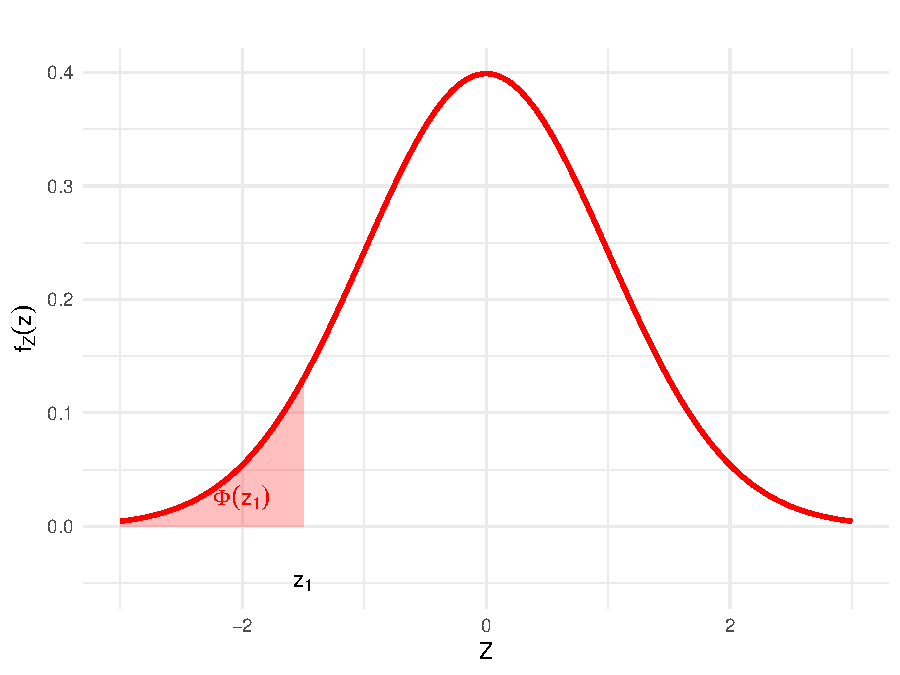
\includegraphics[width=0.5\linewidth]{figure/unnamed-chunk-9-1} 

}



\end{knitrout}
}
\only<3-3>{
\begin{knitrout}
\definecolor{shadecolor}{rgb}{0.969, 0.969, 0.969}\color{fgcolor}

{\centering 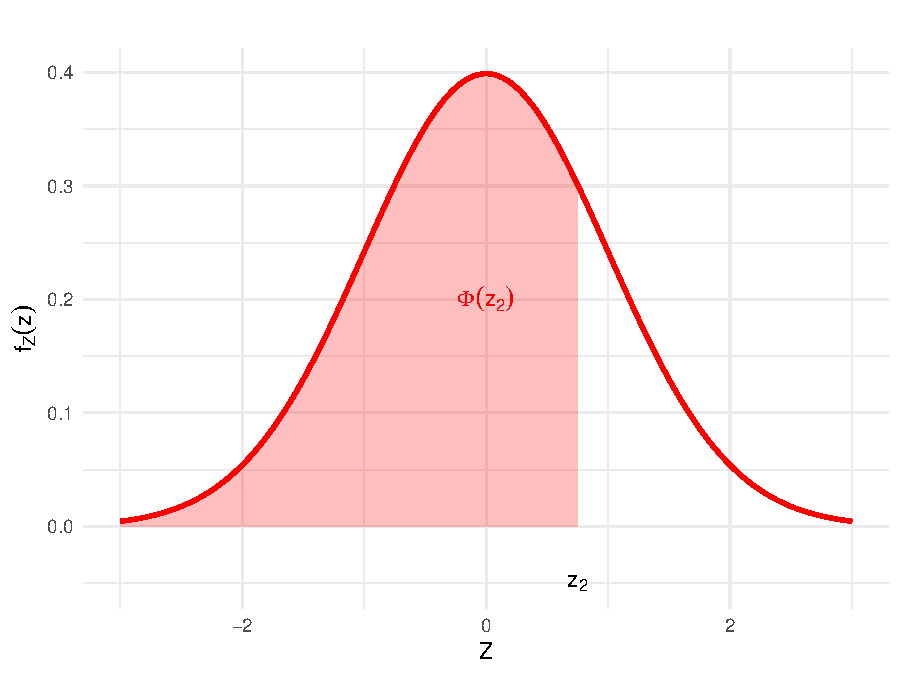
\includegraphics[width=0.5\linewidth]{figure/unnamed-chunk-10-1} 

}



\end{knitrout}
}
\only<4-4>{
\begin{knitrout}
\definecolor{shadecolor}{rgb}{0.969, 0.969, 0.969}\color{fgcolor}

{\centering 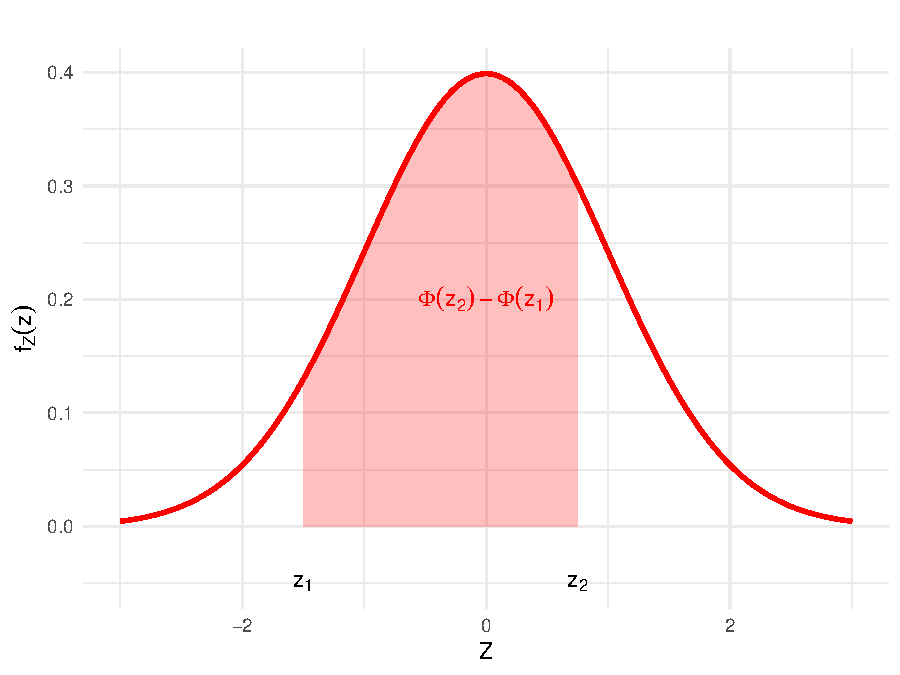
\includegraphics[width=0.5\linewidth]{figure/unnamed-chunk-11-1} 

}



\end{knitrout}
}
\end{frame}


\begin{frame}{\secname}
  \begin{remark}
  The integral that defines the CDF of the standard normal:
    $$
    \Pr(\{Z\leq z\})=\Phi(z)=\int_{-\infty}^z\phi(s)ds
    $$
    \textbf{does not have} a closed-form expression.
  \end{remark}

  \begin{itemize}
    \item It has to be \textbf{approximated using a computer}, e.g. with \texttt{R}.
\begin{knitrout}
\definecolor{shadecolor}{rgb}{0.969, 0.969, 0.969}\color{fgcolor}\begin{kframe}
\begin{alltt}
\hlkwd{pnorm}\hlstd{(}\hlnum{1.924}\hlstd{,} \hlkwc{mean} \hlstd{=} \hlnum{0}\hlstd{,} \hlkwc{sd} \hlstd{=} \hlnum{1}\hlstd{)}
\end{alltt}
\end{kframe}
\end{knitrout}
    \item We can read $\Phi(z)$ for $z\geq 0$ from \textbf{Standard Normal Tables}
  \end{itemize}
  \pause
  \begin{remark}
     We can obtain $\Phi(z)$ for $z < 0$ by symmetry of $\phi(z)$ which, again, entails:
     $$\Phi(-z)=1-\Phi(z)$$
  \end{remark}
\end{frame}

\begin{frame}{\secname}
Description of the values contained in the table:
  \begin{figure}[ptb]\centering
  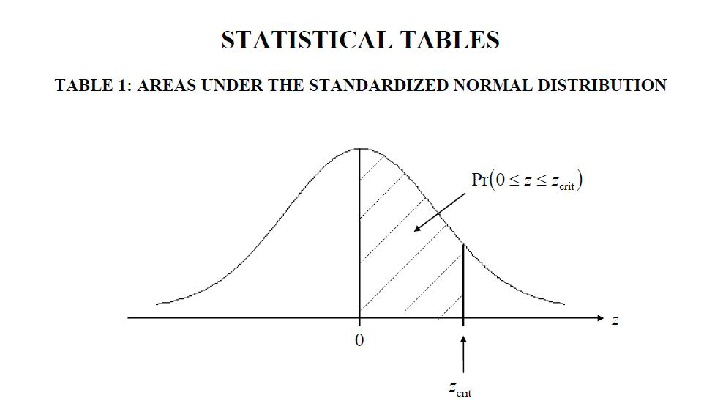
\includegraphics[width=0.95\textwidth,height=0.75\textheight]{img/bell_curve__5.pdf}
  \end{figure}
\end{frame}


\begin{frame}{\secname}
Contents of the table
  \begin{figure}[ptb]\centering
  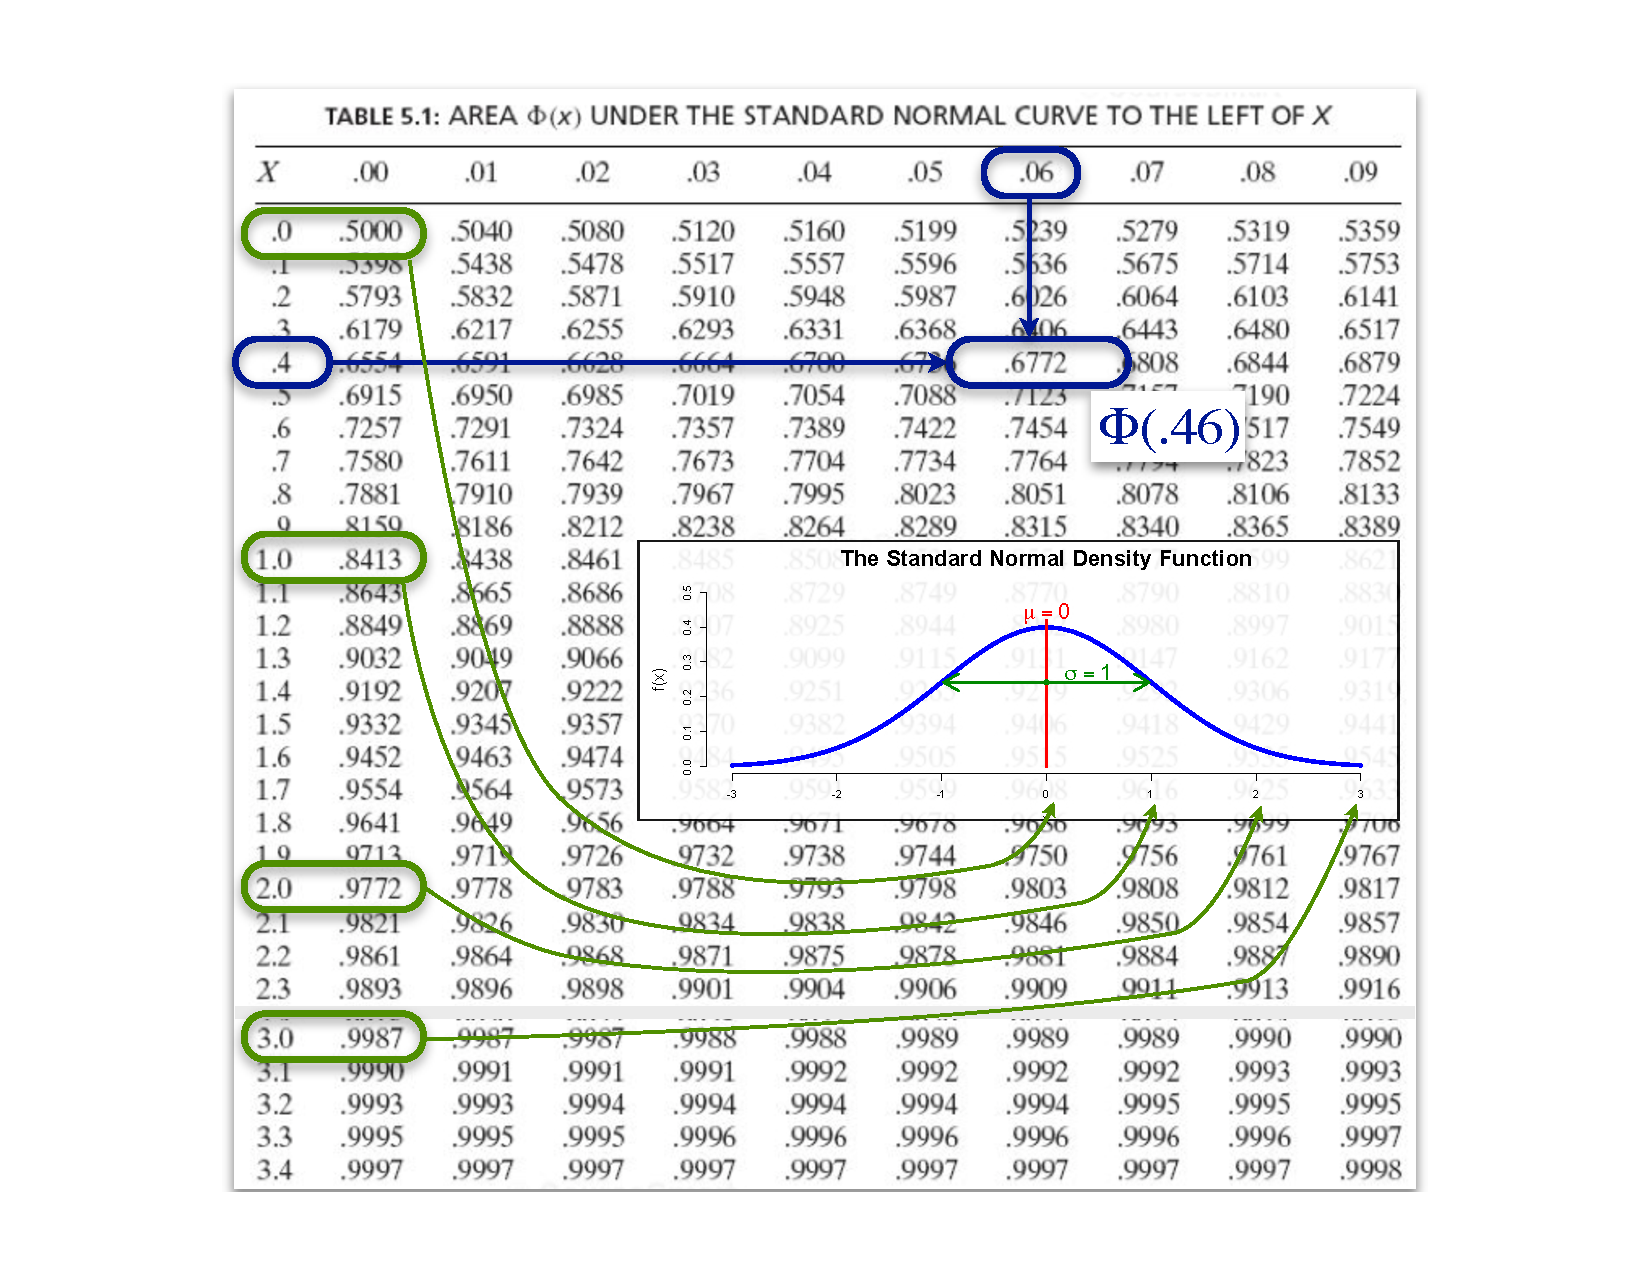
\includegraphics[width=0.9\textwidth,height=0.95\textheight]{img/myTableGauss.pdf}
  \end{figure}
\end{frame}

\begin{frame}{\secname}
  One can use these tables to compute integrals/probabilities of the type:
  \begin{figure}[ptb]\centering
  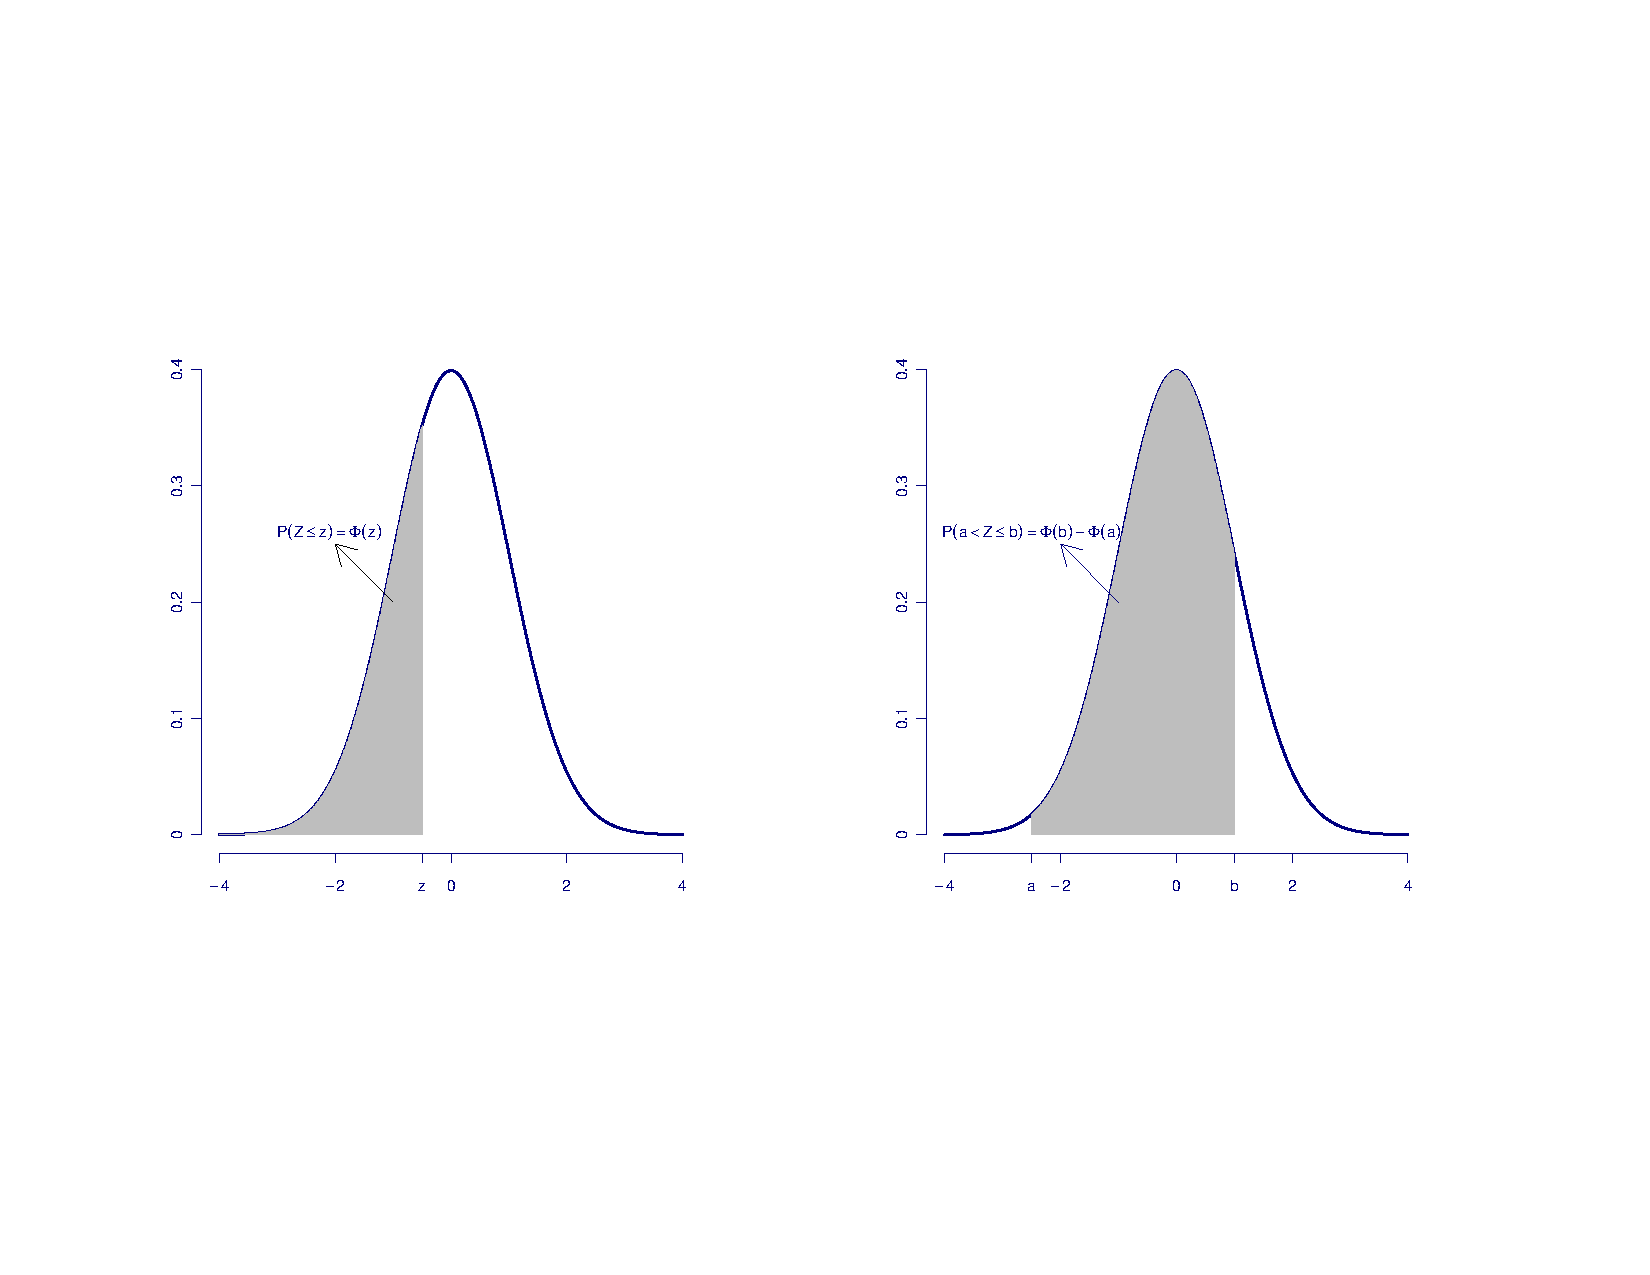
\includegraphics[height=2in, width=4in]{img/CDF_pr.pdf}%
  \end{figure}
\end{frame}

\begin{frame}{\secname}
%\frametitle{Standard Normal Tables}

\begin{example}[Prob of $Z$]
\begin{footnotesize}
  \begin{align*}
  P(\{Z\leq 1\})& \approx0.8413 \\[0.4em]
  P(\{Z\leq 1.96\})& \approx0.9750 \\[0.4em]
  P(\{Z\geq 1.96\})& =1-P(\{Z\leq 1.96\}) \approx 1-0.9750=0.0250 \\[0.4em]
  P(\{Z\geq -1\})& =P(\{Z\leq 1\})\approx 0.8413  \\[0.4em]
  P(\{Z\leq -1.5\})& =P(\{Z\geq 1.5\}) =1-P(\{Z\leq 1.5\}) \approx 1-0.9332=0.0668
  \end{align*}
  \end{footnotesize}
  \end{example}
\end{frame}%

\begin{frame}{\secname}
  %\frametitle{Standard Normal Tables}

  \begin{example}[continued]
  \begin{footnotesize}
  \begin{align*}
  P(\{0.64\leq Z\leq 1.96\}) &= P(\{Z\leq 1.96\})-P(\{Z\leq 0.64\})\\
  & \approx 0.9750-0.7389=0.2361\\[0.5em]
  P(\{-0.64\leq Z\leq 1.96\}) &= P(\{Z\leq 1.96\})-P(\{Z\leq -0.64\})\\
  &=P(\{Z\leq 1.96\})-[\color{blue}{1-P(\{Z\leq 0.64\})}] \\
  &\approx 0.9750-(1-0.7389)=0.7139  \\[0.5em]
  P(\{-1.96\leq Z\leq -0.64\}) &= P(\{0.64\leq Z\leq 1.96\}) \\
  &\approx 0.2361
  \end{align*}
  \end{footnotesize}
  \end{example}
\end{frame}%

\begin{frame}{\secname}
%\frametitle{Normal: an example}

\begin{example}
\begin{footnotesize}
    On the highway A2 (in the Luzern area), the speed is limited to $80$ $km/h$. A radar measures the speeds of all the cars.
    Assuming that the registered speeds are distributed according to a Normal law with mean $72$ $km/h$ and standard error $8$ $km/h$: \vspace{0.2cm}

  \only<1-1>{What is the proportion of the drivers who will have to pay a penalty for high speed?}

  \only<2->{\textit{What is the \textbf{probability} that a driver who will roll at a \textbf{speed $> 80$}}\bigskip}

  \only<3->{
    Let $X$ be the random variable expressing the registered speed: $X \sim \mathcal{N}(72,64)$.\medskip

    Since a driver has to pay if its speed is above $80$ $km/h$, the proportion of drivers paying a penalty is expressed  through $P(X>80)$:
      \begin{equation*}
      P(X>80)= P\left(Z>\frac{80-72}{8} \right)=1-\Phi(1) = 1- 0.8413 = 0.1587
      \end{equation*}
      where $Z \sim \mathcal{N}(0,1)$.\medskip

      Hence, the proportion will be around 16\%
  }
\end{footnotesize}
\end{example}
\end{frame}


\begin{frame}{\secname}
  %\frametitle{Some properties of the Normal distribution}
  In particular, lets consider the probabilty of intervals of the form:
  $$P(\{\mu-\textcolor{red}{k} \sigma \leq X  \leq \mu+\textcolor{red}{k} \sigma\})$$
  for a factor $k \in $
  \begin{figure}[ptb]\centering
  \ \hspace{0.6cm} $\color{red}{k=1}$ \hspace{2.4cm} $\color{red}{k=2}$ \hspace{2.5cm} $\color{red}{k=3}$ \hspace{3cm}
  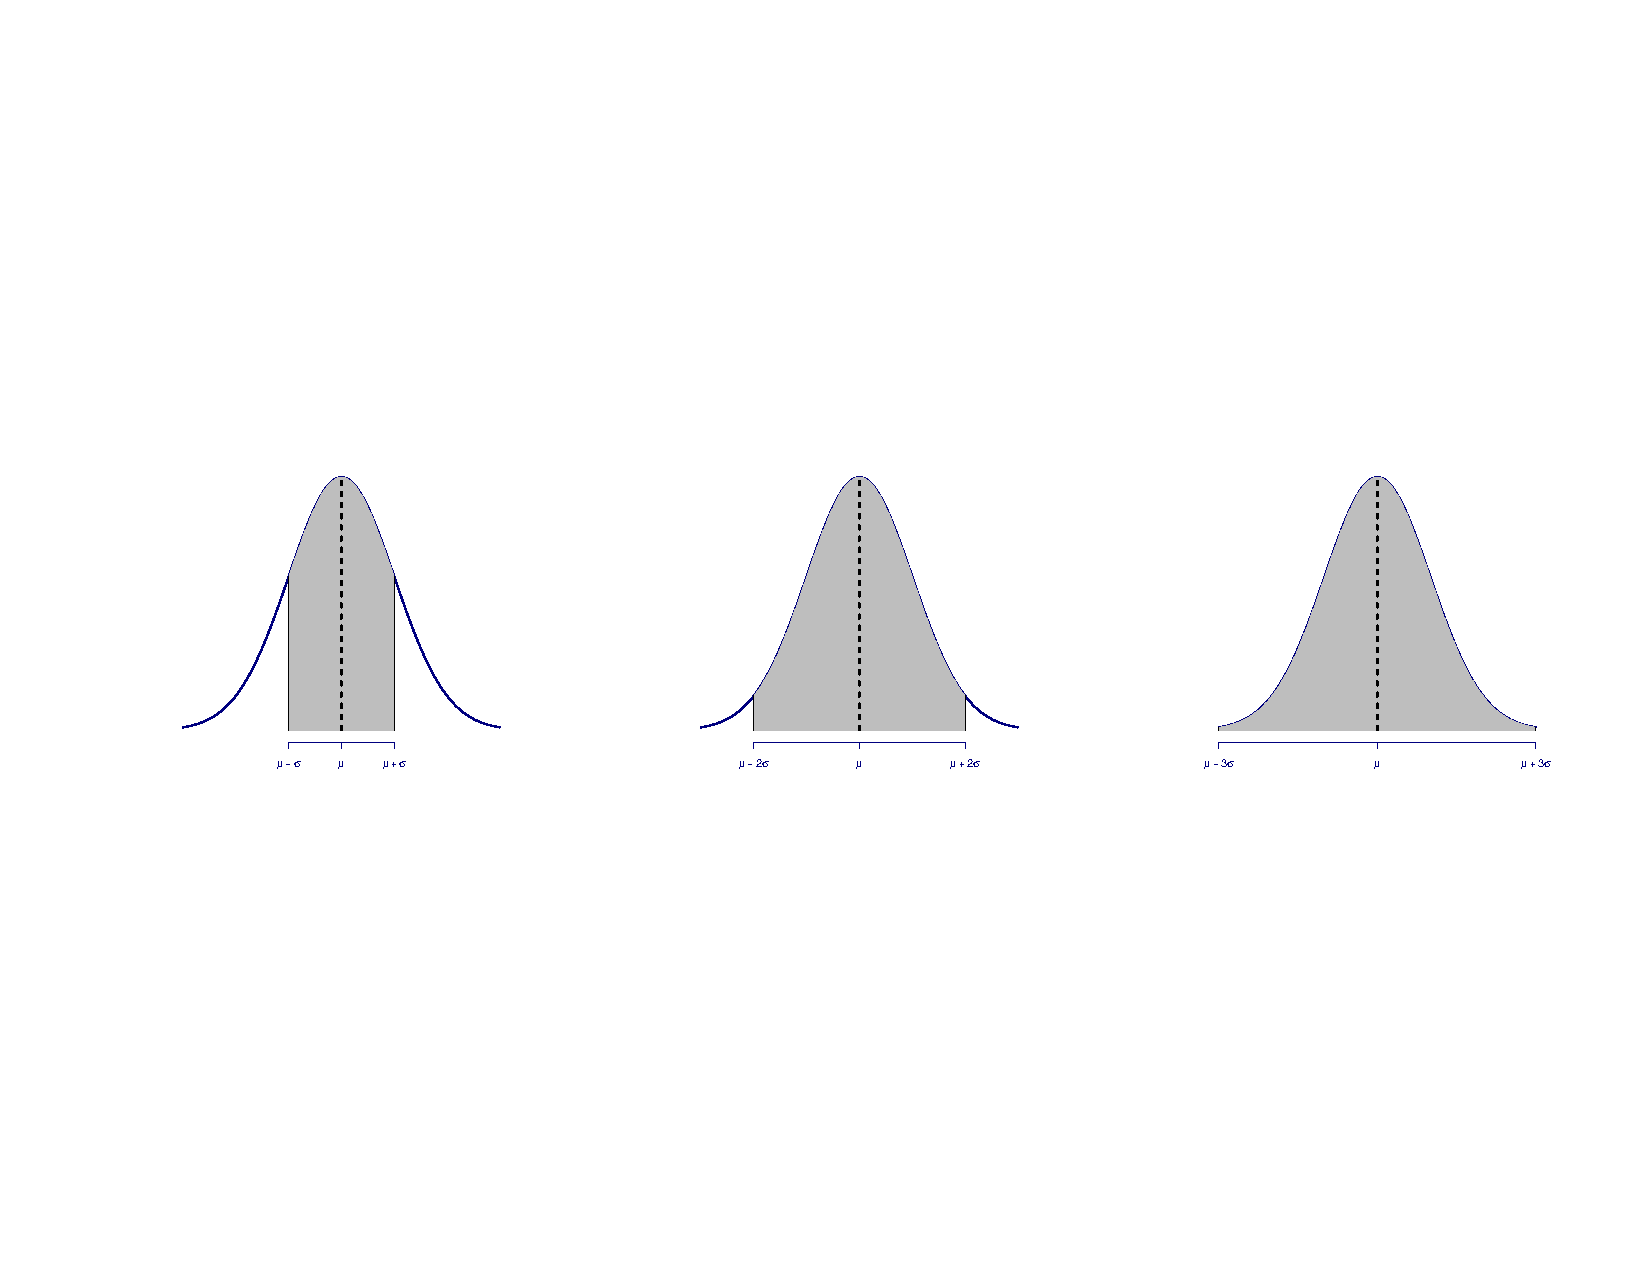
\includegraphics[height=1.5in, width=4.5in]{img/Areas_Normal.pdf}%
  \end{figure}%
  It can be seen that the shaded areas under the pdfs are (approximately) equivalent to $\mathbf{0.683}$, $\mathbf{0.954}$ and $\mathbf{0.997}$,
  respectively.
\end{frame}

\begin{frame}{\secname}
  %\frametitle{Some properties of the Normal distribution}

  \begin{definition}[Rule `68 -- 95 -- 99.7']
  If $X$ is a Normal random variable, $X \sim \N(\mu, \sigma^2)$, its realization has approximately a probability of \\ \bigskip

  \begin{tabular}{llll}
  $\bullet$
  &
  $68 \, \%$
  &
  \mbox{of being in the interval}
  &
  $\lbrack \mu - \sigma, \, \mu + \sigma \rbrack$;\\[0.2cm]
  $\bullet$
  &
  $95 \, \%$
  &
  \mbox{of being in the interval}
  &
  $\lbrack \mu - 2 \, \sigma, \, \mu + 2 \, \sigma \rbrack$;\\[0.2cm]
  $\bullet$
  &
  $99.7 \, \%$
  &
  \mbox{of being in the interval}&
  $\lbrack \mu - 3 \, \sigma, \, \mu + 3 \, \sigma \rbrack$.\\[0.2cm]
  \end{tabular}
  \end{definition}
\end{frame}


\begin{frame}{\secname}
  %\frametitle{Some properties of the Normal distribution}

  \begin{stepitemize}
  \item \textbf{Expectation and Variance} \medskip

  For $X\sim \N\left( \mu ,\sigma ^{2}\right)$
  \begin{equation*}
  E\left[ X\right] =\mu \text{ and }Var\left( X\right) =\sigma ^{2}.
  \end{equation*}

  \item \textbf{Linear Transformations} \medskip

  If $a$ is a number, then
  \begin{eqnarray*}
  X+a &\sim &\N\left( \mu +a,\sigma ^{2}\right) \\
  aX &\sim &\N\left( a\mu ,a^{2}\sigma ^{2}\right).
  \end{eqnarray*}

  \item \textbf{Sum of two Independent Normal RV's} \medskip

  If $X\sim \N\left( \mu ,\sigma ^{2}\right) $ and $Y\sim \N\left( \alpha
  ,\delta ^{2}\right) $, and $X$ and $Y$ are \textbf{independent} then%
  \begin{equation*}
  X+Y\sim \N\left( \mu +\alpha ,\sigma ^{2}+\delta ^{2}\right).
  \end{equation*}
  \end{stepitemize}
\end{frame}


\begin{frame}{\secname}
%\frametitle{The sum of two independent Normals}
  \begin{figure}[ptb]\centering
  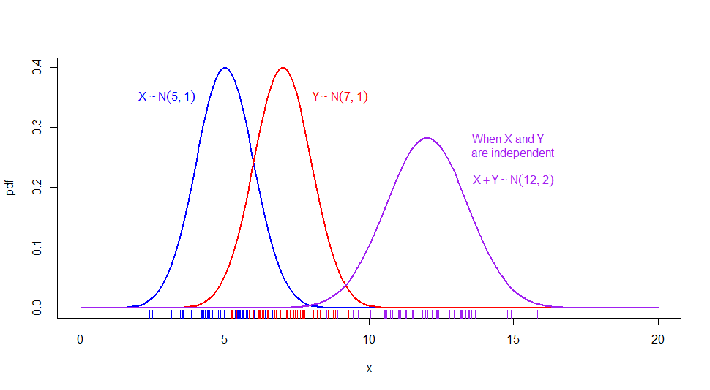
\includegraphics[width=0.95\textwidth,height=0.7\textheight]{img/sum_of_two_independent_normals_with_rug__1.pdf}%
  \end{figure}
  Locations of $n=30$ sampled values of $X,$ $Y$, and $X+Y$ shown as tick marks under each respective density.
\end{frame}


\begin{frame}{\secname}
%\frametitle{Normal: an example}

\begin{example}
\begin{footnotesize}
  On the highway A2 (in the Luzern area), the speed is limited to $80$ $km/h$. A radar measures the speeds of all the cars.
  Assuming that the registered speeds are distributed according to a Normal law with mean $72$ $km/h$ and standard error $8$ $km/h$: \bigskip

\only<1-1>{Knowing that in addition to the penalty, a speed higher than $30$ $km/h$ (over the max allowed speed) implies a withdrawal of the driving license, what is the proportion of the drivers who  will lose their driving license among those who will have a to pay a fine? \medskip}
\only<2->{We are looking for the conditional probability of a recorded speed greater than 110 \underline{given that} the driver has had already to pay a fine:
    \begin{eqnarray*}
    P(X>110 \vert X>80) &=&  \frac{P(\{X>110\} \bigcap \{X>80\})}{P(X>80)} \\
    &=& \frac{P(X>110)}{P(X>80)} = \frac{1- \Phi((110-72)/8)}{1-\Phi(1)}\approx \frac{0}{16\%}\simeq 0.
    \end{eqnarray*}
    }
\end{footnotesize}
\end{example}
\end{frame}





%%%%%%%%%%%%%%%%%%%%%%%%%%%%%%%%%%%%%%%%%%%%%%%%%%%%%%%%%%%%%%%%%%%%%%%%%%%%%%%%
\section{The Chi-squared distribution}
%%%%%%%%%%%%%%%%%%%%%%%%%%%%%%%%%%%%%%%%%%%%%%%%%%%%%%%%%%%%%%%%%%%%%%%%%%%%%%%%

\begin{frame}{\secname}
  \begin{definition}
  If $Z_{1},Z_{2},\ldots ,Z_{n}$ are independent standard Normal random
  variables, then%
  \begin{equation*}
  X=Z_{1}^{2}+Z_{2}^{2}+\cdots +Z_{n}^{2}
  \end{equation*}%
  has a chi-squared distribution with $n$ degrees of freedom. Write as $X\sim \chi ^{2}(n)$.
  \end{definition}
\pause
\begin{remark}
  $X\sim \chi ^{2}(n)$ can take only \textbf{positive }values. Moreover, expected value and variance, for $X\sim \chi ^{2}(n)$, are:
  \begin{eqnarray*}
  E\left[ X\right] &=&n \\
  Var\left( X\right) &=&2n
  \end{eqnarray*}
\end{remark}
\begin{remark}
  If $X\sim \chi ^{2}(n)$ and $Y\sim \chi ^{2}(m)$ are \textbf{independent} then $X+Y\sim \chi ^{2}(n+m)$.
\end{remark}
\end{frame}

\begin{frame}{\secname}

\begin{figure}[ptb]\centering
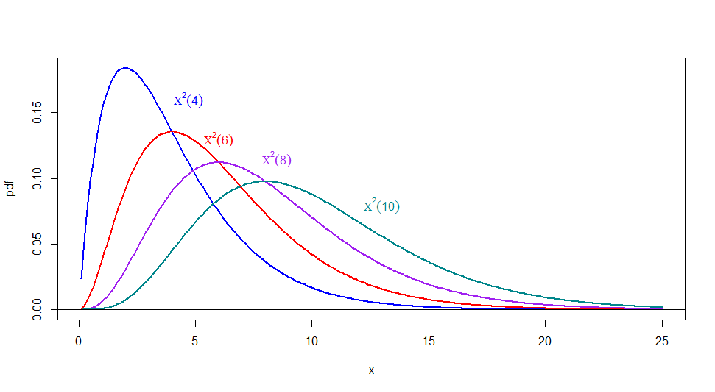
\includegraphics[height=2.6143in, width=4.6643in]{img/chisquared_pdfs__2.pdf}%
\end{figure}

\emph{Quantiles} for Chi-squared probabilities may be read from a table.

\end{frame}%

\begin{frame}{\secname}

%\frametitle{Chi-squared table}


\begin{figure}[ptb]\centering
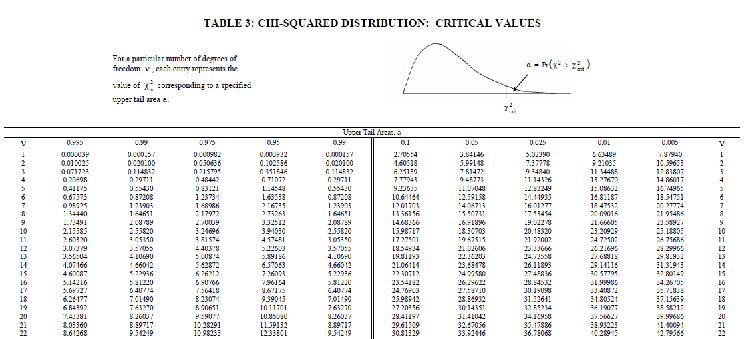
\includegraphics[height=2.2649in, width=4.9658in]{img/chisq_table__3.pdf}%
\end{figure}

\end{frame}%

\begin{frame}{\secname}
%\frametitle{Chi-squared table (illustration of its use)}

\begin{example}
  \begin{footnotesize}
  Let $X$ be a chi-squared random variable with 10 degrees-of-freedom. What is the value of its \underline{upper fifth percentile}? \bigskip

  By definition, the upper fifth percentile is the chi-squared value $x$ (lower case!!!) such that the probability to the right of $x$ is $0.05$ (so the upper tail area is $5\%$).  To find such an $x$ we use the chi-squared table: \medskip
  \begin{itemize}
  \item setting $\mathcal{V} = 10$ in the first column on the left and getting the corresponding row \medskip
  \item finding the column headed by $P(X \geq x) = 0.05$. \medskip
  \end{itemize}

  Now, all we need to do is read the corresponding cell. What do we get? Well, the table tells us that the upper fifth percentile of a chi-squared random variable with 10 degrees of freedom is \textbf{18.30703}.
  \end{footnotesize}
\end{example}
\end{frame}

%%%%%%%%%%%%%%%%%%%%%%%%%%%%%%%%%%%%%%%%%%%%%%%%%%%%%%%%%%%%%%%%%%%%%%%%%%%%%%%%
\section{The Student-t distribution}
%%%%%%%%%%%%%%%%%%%%%%%%%%%%%%%%%%%%%%%%%%%%%%%%%%%%%%%%%%%%%%%%%%%%%%%%%%%%%%%%

\begin{frame}{\secname}
  \begin{definition}
  If $Z\sim \N(0,1)$ and $Y\sim \chi ^{2}(v)$ are \textbf{independent}
  then%
  \begin{equation*}
  T=\frac{Z}{\sqrt{Y/v}}
  \end{equation*}%
  has a \textbf{Student-t} distribution with $v$ degrees of freedom. Write as $T\sim t_{v}$.
  \end{definition}
  \bigskip
  $T\sim t_{v}\,$\ can take any value in $\mathbb{R}$. Expected value and variance for $T\sim t_{v}$ are
  \begin{eqnarray*}
  E\left[ T\right] &=&0\text{, for }v>1 \\
  Var\left( T\right) &=&\frac{v}{v-2}\text{, for }v>2.
  \end{eqnarray*}
\end{frame}

\begin{frame}{\secname}
  \begin{remark}
  The pdf of $T\sim t_{v}$ is similar to a Normal (with mean zero) but with fatter tails. When $v$ is large (typically, $v \geq 120$) $t_{v}$ approaches $\N(0,1)$.
  \end{remark}

  \begin{figure}[ptb]\centering
  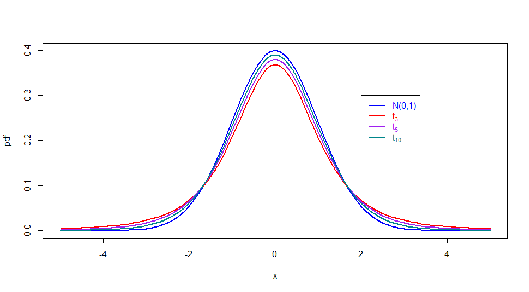
\includegraphics[height=1.9398in, width=3.5345in]{img/student_t__4.pdf}%
  \end{figure}
\end{frame}

\begin{frame}{\secname}
%\frametitle{Student-t table}

\begin{figure}[ptb]\centering
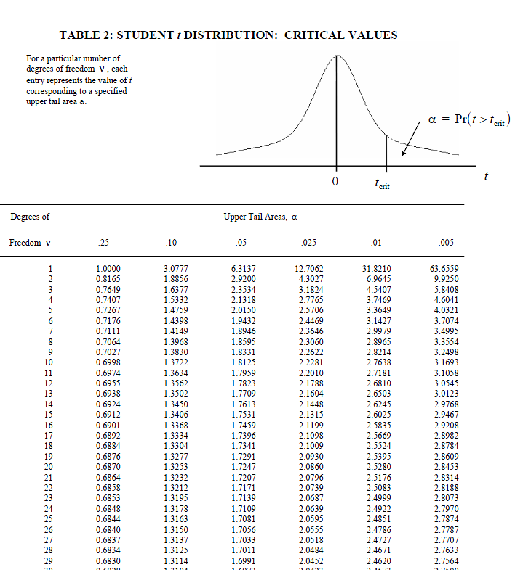
\includegraphics[height=3.8in, width=3.506in]{img/Student_t_table__5.pdf}%
\end{figure}

\end{frame}

%%%%%%%%%%%%%%%%%%%%%%%%%%%%%%%%%%%%%%%%%%%%%%%%%%%%%%%%%%%%%%%%%%%%%%%%%%%%%%%%
\section{The F distribution}
%%%%%%%%%%%%%%%%%%%%%%%%%%%%%%%%%%%%%%%%%%%%%%%%%%%%%%%%%%%%%%%%%%%%%%%%%%%%%%%%

\begin{frame}{\secname}
  \begin{definition}
  If $X\sim \chi ^{2}(v_{1})$ and $Y\sim \chi ^{2}(v_{2})$ are \textbf{%
  independent}, then%
  \begin{equation*}
  F=\frac{\frac{X}{v_{1}}}{\frac{Y}{v_{2}}},
  \end{equation*}%
  has an \textbf{F} distribution with $v_{1}$ `numerator' and $v_{2}$
  `denominator' degrees of freedom. Write as $F\sim F_{v_{1},v_{2}}$.
  \end{definition}

  $F\sim F_{v_{1},v_{2}}\,$\ can take only \textbf{positive }values. Expected value and variance for $F\sim F_{v_{1},v_{2}}$ (note that the order of the degrees of freedom is important!).
  \begin{eqnarray*}
  E\left[ F\right] &=&\frac{v_{2}}{v_{2}-2}\text{, for }v_{2}>2 \\
  Var\left( F\right) &=&\frac{2v_{2}^{2}\left( v_{1}+v_{2}-2\right) }{%
  v_{1}\left( v_{2}-2\right) ^{2}\left( v_{2}-4\right) }\text{, for }v_{2}>4.
  \end{eqnarray*}
\end{frame}

\begin{frame}{\secname}
  %\frametitle{Some F distributions}

  \begin{figure}[ptb]\centering
  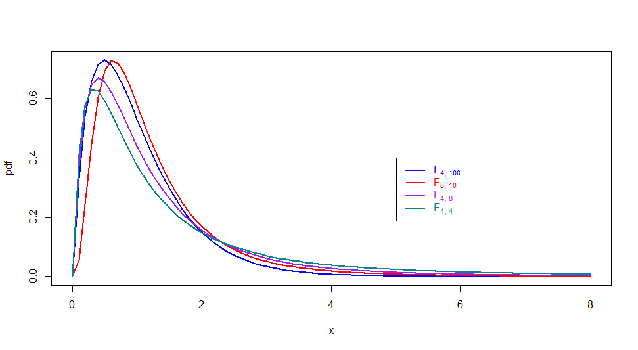
\includegraphics[height=2.3324in, width=4.2462in]{img/F-dist_pds__6.pdf}%
  \end{figure}%
\end{frame}%

\begin{frame}
  %\frametitle{F distribution table (5\% upper tail)}
  \begin{figure}[ptb]\centering
  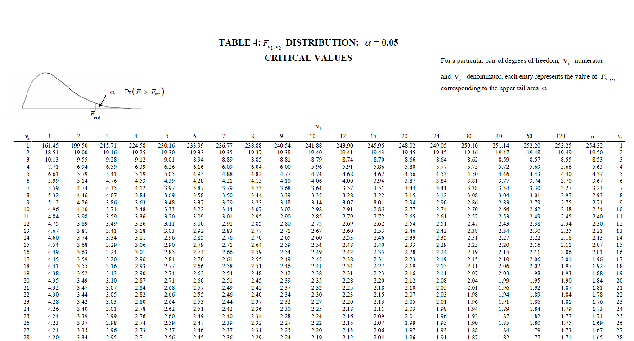
\includegraphics[height=2.2753in, width=4.2263in]{img/Fdist_table__7.pdf}%
  \end{figure}
\end{frame}%

%%%%%%%%%%%%%%%%%%%%%%%%%%%%%%%%%%%%%%%%%%%%%%%%%%%%%%%%%%%%%%%%%%%%%%%%%%%%%%%%
\section{The lognormal distribution}
%%%%%%%%%%%%%%%%%%%%%%%%%%%%%%%%%%%%%%%%%%%%%%%%%%%%%%%%%%%%%%%%%%%%%%%%%%%%%%%%

\begin{frame}{\secname}
  \begin{definition}
   $Y$ has a \textbf{lognormal distribution} when
   $$\ln \left( Y\right) =X$$
  has a Normal distribution. We write $Y\sim $ \emph{lognormal}$\left( \mu ,\sigma ^{2}\right) $.
  \end{definition}

  \medskip

  If $Y\sim $ \emph{lognormal}$\left( \mu ,\sigma ^{2}\right) $ then%
  \begin{eqnarray*}
  E\left[ Y\right] &=&\exp{ \left( \mu +\frac{1}{2}\sigma ^{2}\right)} \\
  Var(Y) &=&\exp{ \left( 2\mu +\sigma ^{2}\right)} \left( \exp{ \left( \sigma
  ^{2}\right)} -1\right).
  \end{eqnarray*}
\end{frame}

\begin{frame}{\secname}
  Let us just see some plots... more to come later...
  \begin{figure}[ptb]\centering
  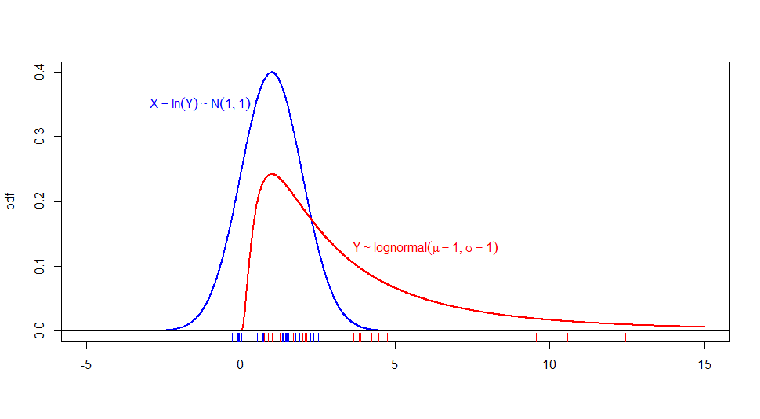
\includegraphics[height=2.4856in, width=4.5in]{img/lognormal_with_rug__8.pdf}%
  \end{figure}
\end{frame}

%%%%%%%%%%%%%%%%%%%%%%%%%%%%%%%%%%%%%%%%%%%%%%%%%%%%%%%%%%%%%%%%%%%%%%%%%%%%%%%%
\section{Exponential distribution}
%%%%%%%%%%%%%%%%%%%%%%%%%%%%%%%%%%%%%%%%%%%%%%%%%%%%%%%%%%%%%%%%%%%%%%%%%%%%%%%%

\begin{frame}{\secname}
  \begin{definition}
  Let $X$ be a  continuous random variable, having the following  characteristics:
  \begin{itemize}
  \item[--]       $X$ is defined on the positive real numbers $\left( 0;\infty \right) $ --- namely $\mathbb{R}^+$;
  \item[--]       the pdf and CDF are
  \bea
  f_X(x)=\lambda \exp\{ -\lambda x\},\lambda
  >0; &
  F_X(x)=1-\exp (-\lambda x); \nn \eea
  \end{itemize}
  then we say that $X$ has an exponential distribution. We write $X\sim$ \text{Exp$(\lambda)$}.
  \end{definition}
\pause
  For $X\sim$ \text{Exp$(\lambda)$} we have that:
  \begin{small}
  \bea
  E[X]=\int_{0}^{\infty }xf_X(x )dx= 1/\lambda & \text{and} &   Var(X)=\int_{0}^{\infty }x^{2}f_X(x )dx-E^{2}(X)=1/\lambda ^{2}. \nn
  \eea
  \end{small}
\pause
  \begin{remark}
  $X$ is typically applied to model the waiting time until an event occurs, when events are always occurring at a random rate $\lambda >0$. Moreover, the sum of independent exponential random variables has a Gamma distribution (see tutorial).
  \end{remark}
\end{frame}

\begin{frame}{\secname}
  %\frametitle{Exponential distribution}
  \begin{small}
  \begin{example}
  Let $X\sim$ \text{Exp}$(\lambda)$, with $\lambda =0.5$. Thus
  $$f_X(x) = \left\{ \begin{array}{ll}
  0.5 \exp (-0.5x) & x>0\\
  0 & \text{otherwise}
  \end{array} \right.$$
  Then, find the CDF.
  \pause
  \medskip

  For $x>0$, we have
  \begin{eqnarray*}
  F_{X}(x) & = & \int_{0}^{x}f_{X}(u)du\\
  & = & 0.5\Big( -2\exp (-0.5u)\Big) \bigl|_{u=0}^{u=x}\\
  & = & 0.5(-2\exp (-0.5x)+2\exp (0))\\
  & = & 1-\exp (-0.5x)
  \end{eqnarray*}
\pause
  so, finally,

  $$F_X(x) = \left\{ \begin{array}{ll}
  0 & x \leq 0 \\
  1-\exp (-0.5x)& x>0
  \end{array} \right.$$
  \end{example}
  \end{small}
\end{frame}

\begin{frame}{\secname}
  \begin{example} [continued]

  and a graphical illustration, with varying $\lambda$

  % \begin{figure}[ptb]\centering
  % 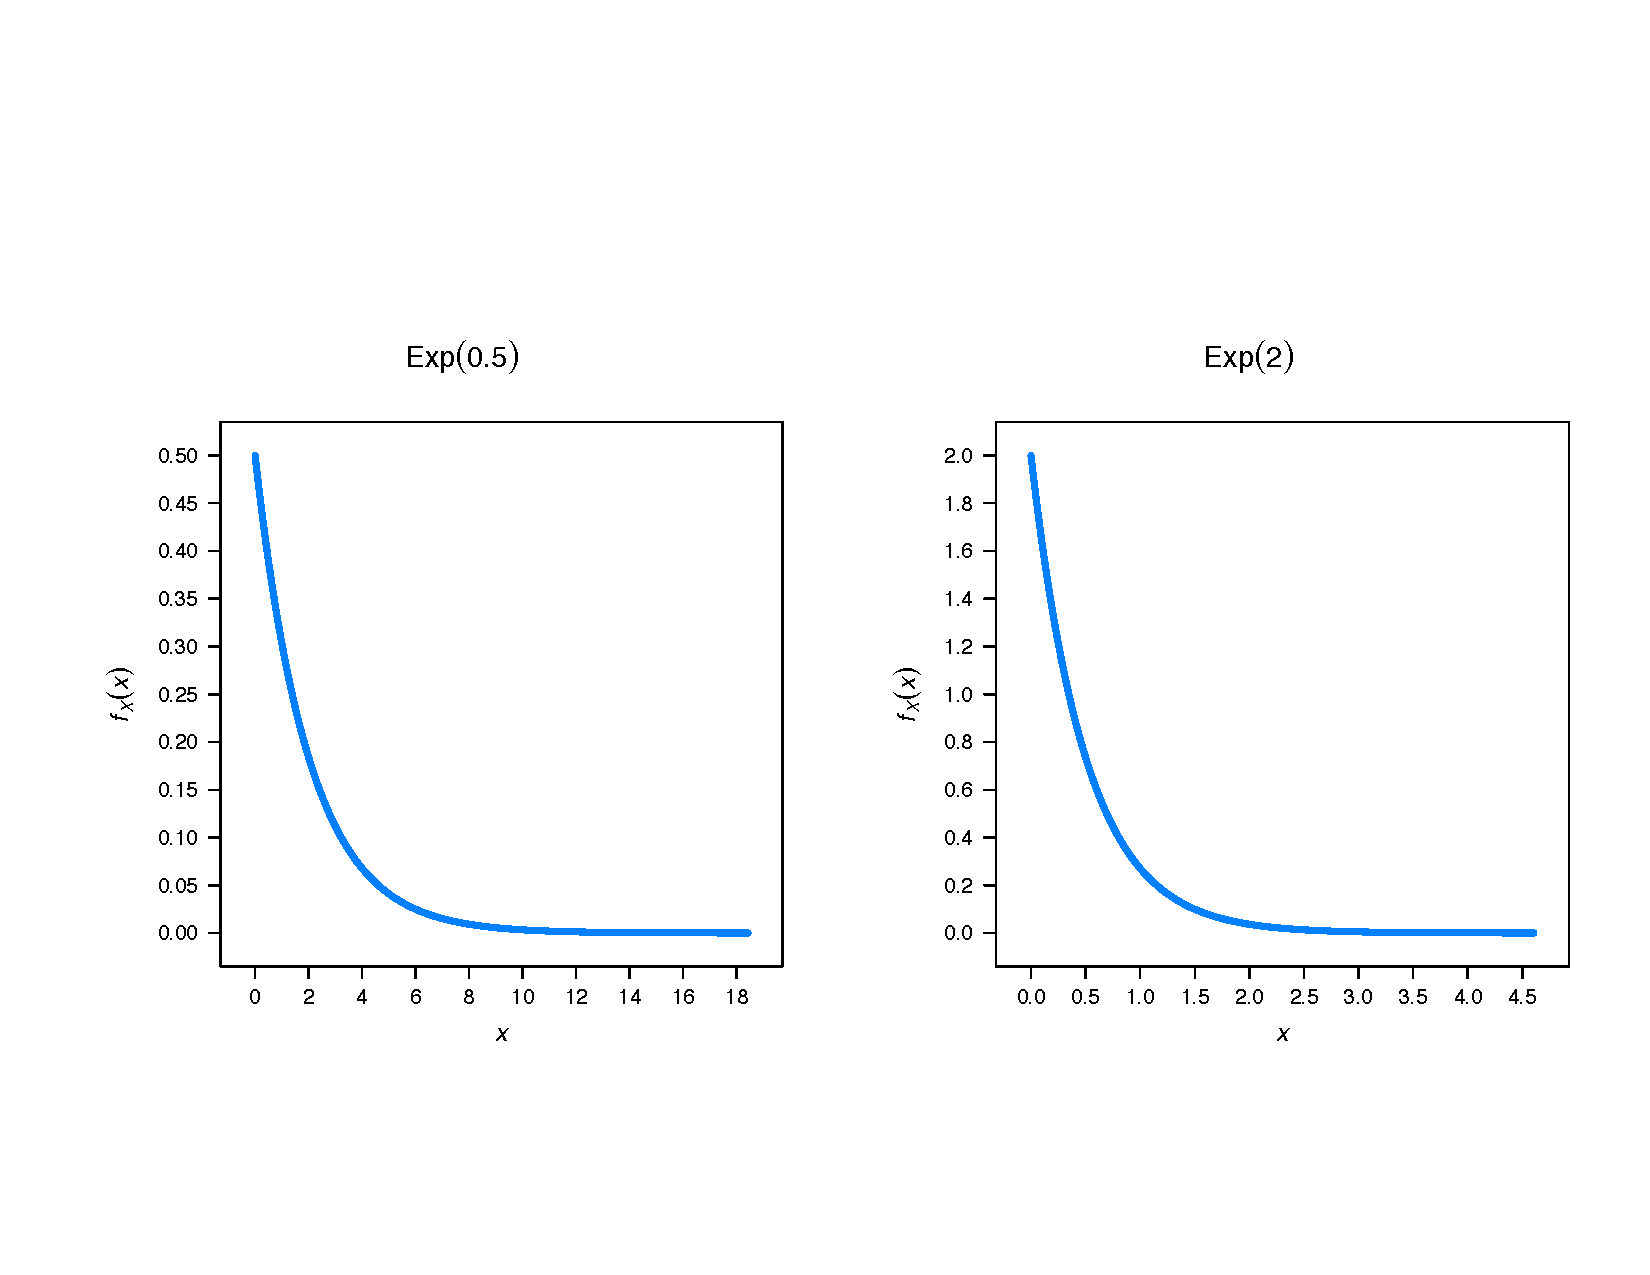
\includegraphics[height=2.4856in, width=4.5in]{img/Exp_Diego.pdf}%
  % \end{figure}
\begin{knitrout}
\definecolor{shadecolor}{rgb}{0.969, 0.969, 0.969}\color{fgcolor}

{\centering 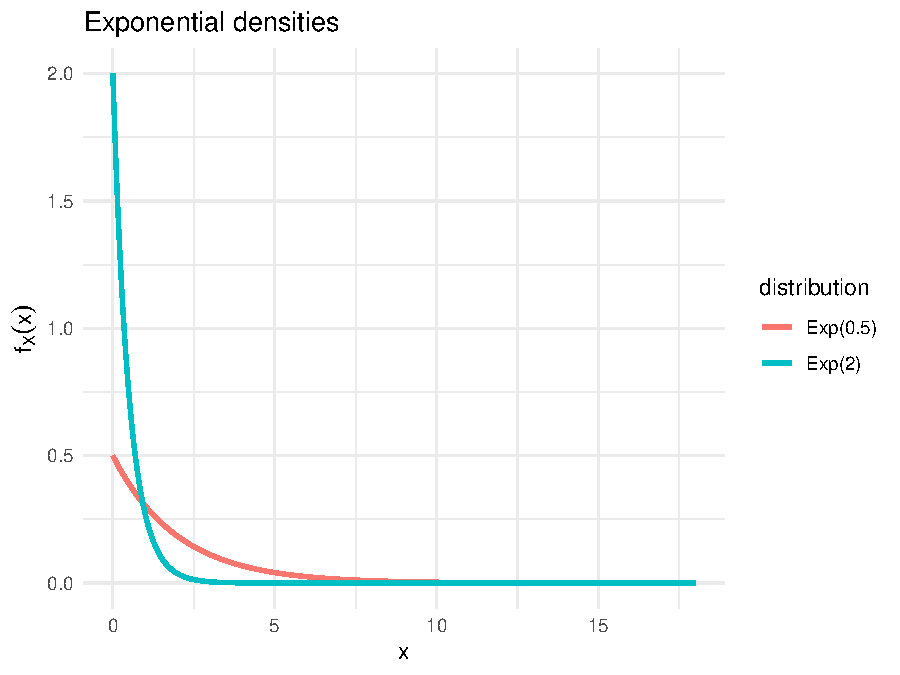
\includegraphics[width=0.5\linewidth]{figure/unnamed-chunk-13-1} 

}



\end{knitrout}

  \end{example}
\end{frame}

\begin{frame}{Wrap-up}

\begin{itemize}
\item Properties of any Normal-distributed Random Variable can be figured out by studying the Standard Normal.\bigskip
\item The Standard Normal is at the core of many other important distribution (Chi-Square, Student's, Fisher's F, log-normal) \bigskip
\item The Cumulative Probabilities of a standard normal $Z$ for $z>0$ are in tables, and can help us calculate the probability of any interval for any Normal.  \bigskip
\item The other distributions introduce the notion of \emph{degrees of freedom} and their tables display the \emph{quantiles} for some upper or lower-tail probabilities for distribution with given degrees of freedom.
\end{itemize}


\end{frame}

\begin{frame}
  \begin{center}
  \Large{Thank You for your Attention!}

  \bigskip
  \pause


  \Large{``See you'' Next Week}
  \end{center}
\end{frame}

\end{document}
